%\documentclass[12pt,ascmac]{jreport}
\documentclass[12pt]{jreport}
\usepackage{comment}
\usepackage{./sty/eclepsf}
\usepackage{tascmac}
\usepackage{tabularx}
\usepackage{listliketab}
\usepackage[longnamesfirst]{natbib}
\usepackage[dvipdfmx]{graphics}
\usepackage[dvipdfmx]{graphicx}
\usepackage[dvipdfmx]{color}
\usepackage{subfigure}
\usepackage{alltt}
\usepackage{here}
\usepackage{afterpage}
\usepackage{./sty/ncodeline}
%\usepackage[dvipdfmx, colorlinks, breaklinks,%
\usepackage[dvipdfmx, breaklinks,%
bookmarks=true, bookmarksnumbered=true,%
bookmarkstype=toc, bookmarksopen=true,bookmarksopenlevel=3,%
pdftitle={Improve the Readability of Swift Compiler by Self-hosting},%
%%pdfsubject={},%
pdfauthor={Atsuki Demizu},%
pdfkeywords={1.Compiler, 2.Self-hosting, 3.Readability of Program, 4.Swift Programming Language}%
]{hyperref}
\usepackage{bookmark}

\AtBeginDvi{\special{pdf:tounicode EUC-UCS2}}

\usepackage{fancyhdr}

\usepackage{./sty/doxygenorig}

\usepackage{indentfirst}
\usepackage{url}
\usepackage{listings,./sty/jlisting}

\def\lstlistingname{プログラム}

\lstset{%
 language={C++},
 %backgroundcolor={\color[gray]{.85}},%
 basicstyle={\small\ttfamily},%
 identifierstyle={\small},%
 commentstyle={\small\itshape},%
 keywordstyle={\small\bfseries},%
 ndkeywordstyle={\small\ttfamily},%
 stringstyle={\small\ttfamily},
 frame={tb},
 framesep=1zw,
 breaklines=true,
 numbers=left,%
 xrightmargin=0zw,%
 xleftmargin=1.5zw,%
 numberstyle={\scriptsize},%
 stepnumber=1,
 numbersep=1zw,%
 lineskip=-0.5ex%
}

\usepackage{amssymb}
%\usepackage{supertabular,multirow}

\usepackage{array}
\newcolumntype{M}[1]{>{\centering\arraybackslash}m{#1}}

% A4  size: 297mm*210mm %1pt = 0.35mm
\setlength{\topmargin}{-3.4mm} % 10pt 25.4mm - 3.4mm = 22mm
\setlength{\oddsidemargin}{-0.4mm} % 25.4mm - 0.4mm = 25mm
\setlength{\evensidemargin}{-0.4mm} % 25.4mm - 0.4mm = 25mm
\setlength{\textheight}{231mm} % 660pt % original is 225.75mm 645pt
\setlength{\textwidth}{160mm} % 457pt

\renewcommand{\topfraction}{.99}
\renewcommand{\textfraction}{.0}
\renewcommand{\floatpagefraction}{.99}
\renewcommand{\bibname}{参考文献}

\pagestyle{fancy}
%\rhead{\thepage}
%\rhead[]{\leftmark}
\lhead[]{}
%\lhead[\rightmark]{}

\makeatletter
\def\chaptermark#1{\markboth {\ifnum \c@secnumdepth>\m@ne
\@chapapp\ \thechapter \@chappos\ \fi #1}{}}
\makeatother

\begin{document}

\pagenumbering{roman}

\begin{titlepage}
  \begin{center}
    \begin{large}
      卒業論文   2015年度(平成27年)\\
      \vspace{24pt}
      Self-host化によるSwiftコンパイラのソースコード可読性の向上
      \end{large}
  \end{center}
  \vspace{40em}
  \begin{flushright}
    \large 慶應義塾大学 環境情報学部\\
    出水 厚輝
  \end{flushright}
\end{titlepage}


\thispagestyle{empty}
卒業論文要旨 - 2015年度 (平成27年度)
\begin{center}
\begin{Large}
\begin{tabular}{|c|} \hline
Self-host化によるSwiftコンパイラのソースコード可読性の向上
\\ \hline
\end{tabular}
\end{Large}
\end{center}
%~ \bigskip ~ \\

オープンソースとなったソフトウェアにおいては、その開発に関わるプログラマの増加とそれに伴うプログラムの修正や機能追加の増加によって、そのソースコードの可読性が拡張やそれに対するレビューの容易さに影響し、プロジェクト自体の成否に大きく関わる場合がある。

2015年12月にオープンソースとなったApple社が中心となって開発しているプログラミング言語Swiftもそうした可能性の分岐点に立つソフトウェアの1つである。
現在Swiftコンパイラの可読性は既存コードのコーディングスタイルへの習慣的な追従とレビューの徹底によって保たれているが、この形だけでは新しいコードの増加やプロジェクトメンバーの交代などによってその可読性が保てなくなる可能性が高い。

一方で、Swiftでは行われていないものの、現在利用されている多くの高級な汎用プログラミング言語では、コンパイル対象となる言語自体でそのコンパイラを記述するSelf-host化がよく行われている。
Self-host化を行うことによるメリットはいくつかあるが、たびたびモチベーションとしてあげられるのは、その可読性における優位点である。
コンパイラを記述する言語とその対象言語が同じになれば開発者はより少ない知識でコンパイラのコードを読むことができる上、初期のコンパイラにおいては、それを記述している言語よりもそのコンパイル対象となっている言語のほうが必ず後発のものであるため、多くの場合により表現力が高く、可読性においてもより高い水準となるからである。

そこで本研究では、Swiftで記述されたSwiftコンパイラの構文解析器を実装し、現行のSwiftコンパイラの構文解析器とそのソースコードの行数を多面的に比較することでSelf-host化がSwiftコンパイラに与える影響についての検証を行った。
検証の結果として、本論文ではSwiftコンパイラのSelf-host化によってその可読性が向上する可能性が十分にあることを示している。
だだし、同時に行ったSelf-host化に伴うデメリットの考察により、Self-host化がコンパイラに対して与える他の影響を鑑みると、実際の適用に際してはより慎重にならなければいけないということもわかった。

~ \\
キーワード:\\
\underline{1. コンパイラ},
\underline{2. Self-host化},
\underline{3. プログラムの可読性},\\
\underline{4. プログラミング言語Swift}
\begin{flushright}
慶應義塾大学 環境情報学部\\
出水 厚輝
\end{flushright}

\clearpage

\thispagestyle{empty}
Abstract of Bachelor's Thesis - Academic Year 2015
\begin{center}
\begin{large}
\begin{tabular}{|p{0.97\linewidth}|}
    \hline
    Improvement of the Readability of Swift Compiler's Source Code by Self-hosting\\
    \hline
\end{tabular}
\end{large}
\end{center}

~ \\

When the software project changes into an open source, as both the number of joining developpers \& the extension/modification of program increase, the readability of software's source code becomes important factor for succeeding the project.

In December 2015, the Swift programming language project, which is leaded by Apple, made its souce code public and started to face with such a change.
In current process, the readability of Swift compiler is maintained just by the effort to habitually follow the coding style of existing codes and its strict review.
Therefore, when the new codes grows wider in the software, its readability should become out of control.

On the other hand, there is a technique called Self-hosting, which is adopted in many general-purpose high-level programming languages.
The Self-hosting is a technique writing the compiler in its targeting programming language.
Although there are multiple reasons to adopt the Self-hosting to the compile, the most attractive advantage is that developers can reduce their effort for understanding the software.
When the compiler is self-hosted, its developpers are not reqired to learn the other than the targeting language.
And furthermore, as the targeting language is newer than its compiler's description language in the early years, the Self-hosting has an effect to change the compiler's source code less complex with the new and expressive grammars of targeting language.

In this research, we implemented the new Swift compiler which is written by Swift and compare its parser with the parser of Apple's Swift compiler in order to verify the readability enhancement ability of Self-hosting.
As the result of this research, we colud confirm the positive effect of Self-hosting on the readability.
But at the same time, as the effect depends on some characteristic grammars of Swift, we are considering that some other languages whose compiler is written by other high-level language may not be benefited the effect.

~ \\
Keywords : \\
\underline{1. Compiler},
\underline{2. Self-hosting},
\underline{3. Readability of Program},\\
\underline{4. Swift Programming Language}
\begin{flushright}
Keio University, Faculty of Environment and Information Studies\\
Atsuki Demizu
\end{flushright}

\clearpage

\tableofcontents\thispagestyle{empty} %目次
\clearpage
\listoffigures\thispagestyle{empty} %図目次
\clearpage
\listoftables\thispagestyle{empty} %表目次
\clearpage
\pagenumbering{arabic}
\chapter{序論}
\label{introduction}

\section{背景}
\label{introduction:background}

2015年12月4日、Apple社が予てより同社の提供するCocoaおよびCocoa Touchフレームワークを用いたソフトウェアの開発用として提供していたプログラミング言語Swiftをオープンソース化し、Linuxを中心としたさまざまなプラットフォームにおけるソフトウェアを開発するための拡張を開始した。
これによりプログラミング言語SwiftはObjective-Cの担ってきたiOSやMac OS Xなどにおけるソフトウェアの開発だけでなく、C++やJavaなど他の汎用プログラミング言語が担ってきたソフトウェア開発においても、それらの代替となり得る可能性を持つこととなった。

Swiftはオブジェクト指向や全称型・存在型の導入、関数の第一級オブジェクト化、HindlyとMilnerによる型再構築アルゴリズムの採用など、現在多くのプログラマに使用されている他の汎用高級言語が持つ様々な特徴を持っているが、まだその特徴を採用するか否かがよく議論されていないものもある。
その内の1つがコンパイラをそのコンパイル対象の言語自体で開発するBootstrapプロセスの採用である。

表~\ref{table:bootstrapping-languages}はWeb検索エンジンにおけるクエリヒット数からプログラミング言語の知名度を格付けしたTIOBE Indexの2015年12月版において上げられている言語の内、汎用言語であるものだけを上位から20言語抽出し、それらの主要なコンパイラがその言語自体で記述されているかを示したものである。
この20言語の内だけでもBootstrapを行っているものが8言語あり、 その中に性能の問題からコンパイラ用の言語として採用されづらいインタプリタ型言語なども含まれていることを考慮すれば、かなりの言語がBootstrapされていることが分かる。
しかし、現在SwiftはC++を用いて開発されており、Bootstrapは行われていない。

現在Swiftにおいては未だ多くの機能が不足しており、他の問題を優先しているためにBootstrapについて大きく取り上げられてはいない。
また、開発者のメーリングリスト~\cite{dev-ml}では特にSwiftコンパイラのバックエンドとして採用されているLLVMのAPIがC++で提供されていることから、SwiftがC++と同様の役割を果たすにはもう少し時間が必要だという意見も上がっている。


しかし、~\ref{explain-bootstrap:merit}節で述べるようにBootstrapを行うことで得られる利益があることが他の言語の事例によって示されている以上、十分な議論なしに現状のSwiftにBootstrapが不要であると判断するのは早計であるといえる。

\begin{table}[tb]
    \begin{center}
        \caption{知名度の高いプログラミング言語のBootstrap状況}
        \begin{tabular}{|c|c|c|c|}
            \hline
            順位 & 言語名 & コンパイラ名 & Bootstrap状況 \\
            \hline
            1 & Java & javac & N (C, C++?) \\
            \hline
            1 & Java & OpenJDK & N (C++, Java) \\
            \hline
            2 & C & gcc & N (C++) \\
            \hline
            2 & C & clang & N (C++) \\
            \hline
            3 & C++ & gcc & Y \\
            \hline
            3 & C++ & clang & Y \\
            \hline
            3 & C++ & Microsoft Visual C++ & Y \\
            \hline
            4 & Python & cpython & N (C) \\
            \hline
            4 & Python & PyPy & Y \\
            \hline
            5 & C\# & Microsoft Visual C\# & N (C++) \\
            \hline
            5 & C\# & .NET Compiler Platform (Roslyn) & Y \\
            \hline
            6 & PHP & Zend Engine & N (C) \\
            \hline
            7 & Visual Basic .NET & Visual Studio & N (C++, C\#) \\
            \hline
            7 & Visual Basic .NET & .NET Compiler Platform (Roslyn) & Y \\
            \hline
            8 & JavaScript & SpiderMonkey & N (C, C++) \\
            \hline
            8 & JavaScript & V8 & N (C++, JavaScript) \\
            \hline
            9 & Perl & perl & N (C) \\
            \hline
            10 & Ruby & Ruby MRI & N (C) \\
            \hline
            12 & Visual Basic & Visual Studio & N (C++, C\#) \\
            \hline
            13 & Delphi/Object Pascal & Delphi & N (?) \\
            \hline
            13 & Delphi/Object Pascal & Free Pascal & Y \\
            \hline
            14 & Swift & swift & N (C++) \\
            \hline
            15 & Objective-C & clang & N (C++) \\
            \hline
            15 & Objective-C & gcc & N (C++) \\
            \hline
            17 & Pascal & Free Pascal & Y \\
            \hline
            17 & Pascal & GNU Pascal & N (C, Pascal) \\
            \hline
            20 & COBOL & GnuCOBOL & N (C, C++) \\
            \hline
            21 & Ada & GNAT & Y \\
            \hline
            22 & Fortran & GNU Fortran & N (C, C++) \\
            \hline
            22 & Fortran & Absoft Fortran Compiler & ? \\
            \hline
            23 & D & DMD & Y \\
            \hline
            24 & Groovy & groovy & N (Java, Groovy) \\
            \hline
        \end{tabular}
        \label{table:bootstrapping-languages}
    \end{center}
\end{table}

% \begin{figure}
%     \begin{center}
%         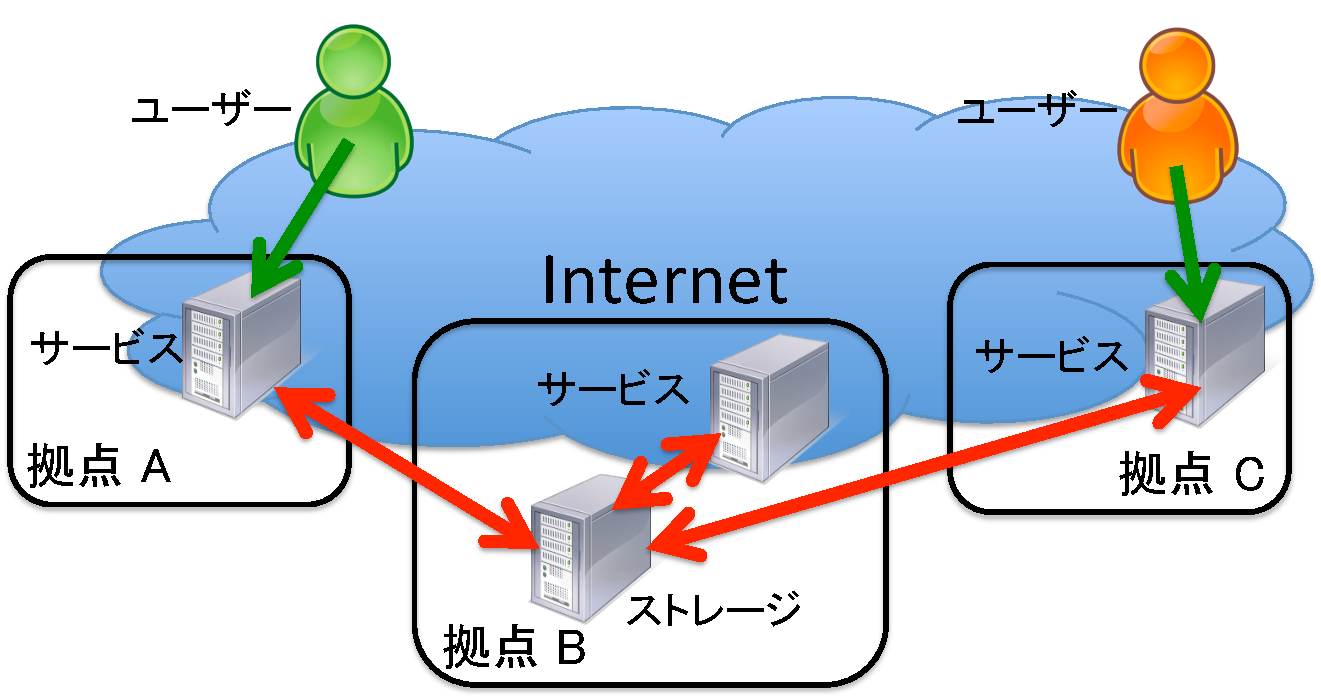
\includegraphics[scale=0.50]{./img/serviceanduser}
%         \caption{複数の拠点から提供されるサービス}
%         \label{img:mlservice}
%     \end{center}
% \end{figure}


\section{本研究が着目する課題}
\label{introduction:issue}

Swiftコンパイラが抱える他の問題との優先度や使用しているフレームワークとのつなぎ込みに関する問題が解決したとしても、SwiftコンパイラのBootstrapを行うかどうかという判断を下すにはより根源的な課題がある。
それは、現在Swiftを記述しているC++言語がSwiftと比較しても高い表現力を持っているために、~\ref{explain-bootstrap:instance}節で見る幾つかの事例とは異なり、Bootstrapを行うことで得られるメリットや、そもそも現行のコンパイラで使用されている手法を維持したままBootstrapを行うことが可能であるか否かが自明でないというものである。

また、現在のSwiftはC++との相互運用性を持っていないため、コンパイラ中の一部分をSwiftで記述したものに置き換えることは難しく、逆に実際に使用されているコンパイラ中のモジュール化が可能なほど大きなパーツをSwiftへ移植するとなると、その間の言語への機能追加などの改変は現行のものと移植中のものの両者に適用するか、移植中のもののみに追加して移植が完了するまでその適用を先送りしなくてはならなくなってしまう。


\section{本研究の目的}
\label{introduction:purpose}

本研究では、SwiftコンパイラがBootstrapすることによって得られるメリットと被るデメリットを定量的に示し、Bootstrapを行うべきか否かを判断する上で有用な情報を収集することを目的とする。
そのためのアプローチとして、Swiftコンパイラの基幹的機能である構文解析器をSwiftによって実装し、その実行時間とソースコードの行数を現行のSwiftコンパイラの構文解析器と比較する。
また、この独自の構文解析器は現行のSwiftコンパイラと基本的な設計手法において同じものを採用するだけで、完全に独立させたものとして実装する。

この方法により、現在のSwiftコンパイラの開発状況などの影響を一切受けずにBootstrapのための評価が可能となり、またその評価がBootstrapの可能性に対して有意義な知見を与えることを提示する。


\section{本論文の構成}

本論文の構成は次の通りである。

第2章では本研究の考察対象であるコンパイラのBootstrapについてSwift以外の言語の事例からそのメリットについてまとめ、Bootstrapにおける課題について整理する。
第3章では本研究が着目するプログラミング言語Swiftの特徴とそのコンパイラ実装の基幹部分における特徴について説明する。
第4章では現行のSwiftコンパイラとの比較対象となるSwiftで記述したSwiftコンパイラ「TreeSwift」の構成について述べ、現行のコンパイラとその基本的な設計手法などに大きな差異がないことを確認する。
第5章では現行のSwiftコンパイラとTreeSwiftの構文解析器についてその実行速度とソースコードの行数を比較し、その結果について考察する。
第6章では本研究の結論と今後の展望についてまとめる。

%%% Local Variables:
%%% mode: japanese-latex
%%% TeX-master: "../thesis"
%%% End:

\chapter{オープンソース化によってSwiftが抱える課題}
\label{open-source}

本章では、本研究の対象とするプログラミング言語であるSwiftが最近行ったオープンソース化の影響についてまとめることで、本研究の着目する課題について整理する。

\section{オープンソースプロジェクトの特徴}
\label{open-source:feature}

オープンソースプロジェクトというプロジェクト形態についてどのようなプロジェクトでなければならないという制約などはないが、特に多くのプロジェクトが従っているオープンソースプロジェクトの持つべき性質がOpen Source Initiativeによって定義されている~\cite{opensource}。
表~\ref{table:open-source-definition}はそのオープンソースの定義をまとめたものである。

\begin{table}[!hbtp]
    \begin{center}
        \caption{オープンソースの定義}
        \begin{tabular}{|p{0.1\linewidth}|p{0.85\linewidth}|}
            \hline
            1 & そのソフトウェア全体を含むソフトウェアの販売・頒布を使用料を課すなどして制限しない \\
            \hline
            2 & ソースコードを利用・改変しやすい形で使用料などを課さずに公開し、その再頒布を制限しない \\
            \hline
            3 & そのソフトウェアの改変・派生および改変・派生したものの同ライセンスでの頒布ができる \\
            \hline
            4 & ソースコードとパッチファイルを共に頒布でき、変更されたソフトウェアの頒布が明確に認められていれば、改変されたソースコードの頒布を制限してもよい \\
            \hline
            5 & 特定の個人や団体を差別しない \\
            \hline
            6 & 利用する分野を制限しない \\
            \hline
            7 & 再頒布されたものであっても、追加の規約などなしにそのプログラムに付随する権利が認められる \\
            \hline
            8 & そのプログラムのライセンスの範囲内で使用・頒布される場合は、プログラムの一部分だけであっても同じ権利が認められる \\
            \hline
            9 & そのソフトウェアと共に頒布されるソフトウェアに対する制限は行わない \\
            \hline
            10 & 特定の技術やインターフェース形式に限定した条件を課さない \\
            \hline
        \end{tabular}
        \label{table:open-source-definition}
    \end{center}
\end{table}

オープンソースプロジェクトはそのソースコードが公開されているために誰でも変更したものを公開できるが、誰もが元々のプロジェクトと全く異なる場所で独自に拡張や修正をしているだけではソフトウェアの発展につながりづらい。
そのため、一般的に多くのオープンソースプロジェクトではその開発プロセス自体をオープンにし、誰もが本体プロジェクトのソフトウェアを拡張・修正できるようになっている。

\begin{table}[!hbtp]
    \begin{center}
        \caption{オープンソースプロジェクトにおける開発フロー}
        \begin{tabular}{|c|p{0.4\linewidth}|p{0.4\linewidth}|}
            \hline
            順序 & 手順 & 具体的な内容の例 \\
            \hline
            \hline
            1 & 任意のユーザからのソフトウェアの拡張や修正提案・要求 & オープンなチケット管理ツールやメーリングリストなどでの拡張・変更提案・バグ報告と議論 \\
            \hline
            2 & 特定の開発者による拡張や修正の実装と提案 & パッチファイルの投稿やPullRequestの作成 \\
            \hline
            3 & 他の開発者による実装へのレビュー & コーディングスタイルや機能の必要性に関する指摘や議論 \\
            \hline
            4 & 修正・拡張の本体ソフトウェアへの統合 & 拡張・修正後のソフトウェアをプロジェクトの最新バージョンとして置き換え \\
            \hline
        \end{tabular}
        \label{table:open-source-flow}
    \end{center}
\end{table}

多くのオープンソースプロジェクトで採用されている開発フローを表~\ref{table:open-source-flow}に示した。
この開発フローは表~\ref{table:open-source-definition}の4番目に該当するバッチファイルによって修正版を公開するような、少し特殊な形式のソフトウェア以外におけるものである。
このように、オープンソースプロジェクトにおける開発では特定組織内のみでの開発とは異なった開発フローとなるという点に注意が必要である。

また、Open Source Initiativeの提唱する定義に合致するオープンソースプロジェクトであっても、そのプロジェクトの形式はそのプロジェクトの方針を決定する主体をどこに置くかによって異なるということをRaymondが自身のエッセイ~\cite{raymond}で提唱している。
表~\ref{table:cathedral-bazaar}に示した「伽藍」と「バザール」という2つの形式である。

\begin{table}[!hbtp]
    \begin{center}
        \caption{Raymondによるオープンソースプロジェクトの分類}
        \begin{listliketab}
        \begin{tabular}{|c|p{0.8\linewidth}|}
            \hline
            形式 & 特徴 \\
            \hline
            \hline
            伽藍形式 & \textbullet \ 中央集権的に開発方針などを指揮し、主な開発を担当する特定集団が存在する \\
            & \textbullet \ 拡張や修正は開発方針に従って行われ、各リリースはよくチェックされる \\
            \hline
            バザール形式 & \textbullet \ 中心的な開発者が指揮者として与える影響は小さく、どの拡張や修正が実施されるかはコミュニティ全体の動向に左右される \\
            & \textbullet \ リリースは変更が加わるごとに更新され、極端に言えばバグを含んだまま行われる \\
            \hline
        \end{tabular}
        \label{table:cathedral-bazaar}
        \end{listliketab}
    \end{center}
\end{table}

伽藍形式のオープンソースプロジェクトはLinux以前の多くのオープンソースプロジェクトで取られていた手法であり、その開発方針は特定の集団によって制御される。
それに対して、Linuxに代表されるバザール形式のオープンソースプロジェクトでは開発者コミュニティの意思によって自然と必要な開発が進められ、プロジェクトの主体となっている個人や団体が開発の各フローにおいて特別に大きな影響力を持たないことを良しとする。

本研究で対象とするSwiftはプロジェクトへの多くの開発者の参加を期待しており、プロジェクトで進められるべき拡張や修正などのほとんどはオープンなメーリングリストやチケッティングツールで決められていくことを望んでいる~\cite{swift-org}。
このことから、Swiftはバザール形式でのプロジェクト展開を目指していると取れるため、本論文では以後バザール形式のオープンソースプロジェクトについてのみ言及する。

最後に、表~\ref{table:open-source-definition}に示したオープンソースプロジェクトの定義と表~\ref{table:cathedral-bazaar}に示したバザール形式の特徴から考えられるバザール形式のオープンソースプロジェクトのそうでないプロジェクトと比較した際の特徴を表~\ref{table:bazaar-features}に整理した。

これらの特徴がバザール形式のオープンソースプロジェクトにおいて、他のプロジェクトにはないメリットやデメリットを提供していると見ることができる。

\begin{table}[!hbtp]
    \begin{center}
        \caption{バザール形式のオープンソースプロジェクトの特徴}
        \begin{listliketab}
        \begin{tabular}{|p{0.35\linewidth}|p{0.6\linewidth}|}
            \hline
            特徴を作る要因 & 特徴 \\
            \hline
            \hline
            様々な人がプログラムを参照する & プログラムのあらゆる箇所に対して任意のタイミングで拡張提案・バグ報告が行われる \\
            \hline
            不特定多数のプログラマが開発に携わる & \textbullet \ プログラムのあらゆる箇所に対して任意のタイミングで拡張・修正が行われる \\
            & \textbullet \ 様々なコーディングスタイルの拡張・修正実装が提案される \\
            \hline
            ソフトウェアを利用したソフトウェアが開発される & ソフトウェアの部分的な利用が試みられる \\
            \hline
            ソフトウェアの技術中立性が高まる & 様々なプラットフォームへの移植が試みられる \\
            \hline
        \end{tabular}
        \label{table:bazaar-features}
        \end{listliketab}
    \end{center}
\end{table}

\afterpage{\clearpage}
\section{クローズドプロジェクトのオープンソース化による変化}
\label{open-source:change}

オープンソースプロジェクトは開発の開始当初からオープンソースプロジェクトとして進められているものと、開発の初期段階ではクローズドだったものが途中からオープンソース化されるものとに分けられる。
初めからオープンソースとなっているプロジェクトでは開発の初期段階でその開発フローなどを徐々に構築していくことが可能となるが、途中からオープンソース化されるプロジェクトではプロジェクトの開発フローや慣習をオープンソース化に合わせて変更していく必要がある。

本説では、~\ref{open-source:feature}節で述べたオープンソースプロジェクトの特徴とクローズドプロジェクトの特徴を比較することでプロジェクトのオープンソース化に伴う変化について整理する。

バザール形式でのオープンソース化を行うと、特に中央管理的に判断されていた開発方針などの事項が開発者コミュニティによって民主的に判断されるようになるという変化が最も大きく、それにともなっていくつかの重要な変化が起こる。
表~\ref{table:open-source-change}はその具体的な変化についてまとめたものである。

\begin{table}[!hbtp]
    \begin{center}
        \caption{バザール形式でのオープンソース化に伴う変化}
        \begin{tabular}{|p{0.25\linewidth}|p{0.35\linewidth}|p{0.35\linewidth}|}
            \hline
            起こる変化 & クローズドプロジェクトでの状況 & オープンソースプロジェクトでの状況 \\
            \hline
            \hline
            拡張や修正の要求・実装が行われるかどうかを決定する要因の変化 & リソースが限られているため、一定の開発方針に従って拡張や修正の優先順位が決定する & ある拡張や修正がそのコストを差し引いても充分な興味を引くものであれば、充分なリソースによって実装されて統合される \\
            \hline
            コーディングスタイルの流動化 & 開発者へのコーディングスタイルの徹底が可能なので同じスタイルを維持することができる & 過去のコードとの統一性も踏まえられるものの、その時々で支持されたコーディングスタイルが用いられるため、スタイルが変動する \\
            \hline
            ソフトウェアの各部分におけるモジュール化 & ソフトウェアの利用先などをすべて把握することが可能なのでモジュール化する部分を限定できる & あらゆる箇所で様々な形でソフトウェアが部分的にも使用されうるため、様々な箇所で高いモジュール性が求められる \\
            \hline
            マルチプラットフォーム化の進行 & 対象とするプラットフォームを制限することができる & 各プラットフォームの熱心なユーザによってマルチプラットフォーム化が進められる \\
            \hline
        \end{tabular}
        \label{table:open-source-change}
    \end{center}
\end{table}

オープンソースプロジェクトではどの拡張や修正を行うかがコミュニティ内の開発者の興味によって決定されるため、コストと照らして充分な価値のある変更には充分なリソースが当てられて取り組まれると期待できるが、それはつまり、拡張や修正のコストが高ければ実装を行うハードルも高くなってしまうということである。
また、コーディングスタイルもクローズドなプロジェクトと比較すると流動化する可能性が高い。
この場合、もちろんより最適なスタイルが選択されていく場合もあるが、ソフトウェア全体で統一したスタイルを徹底することはより難しくなっていくだろう。
クローズドなプロジェクトではそのメリットが限定的になりがちであるモジュール化やマルチプラットフォーム化がそれを所望する熱心な開発者によって進められていく可能性が高いという点は、オープンソースプロジェクトにおけるポジティブな変化と捉えていいだろう。
特にマルチプラットフォーム化は、各プラットフォームの熱心なユーザにとってはその対象ソフトウェアを使用するための必要不可欠な第1歩となるため、特に活発化する可能性が高いとかんがえられる。

ここに挙げた中で最も注目すべき変化は表~\ref{table:open-source-change}中1番上の拡張・修正のコストがある機能を実装するか否かを判断する上で重要な変数となるという点である。
プロジェクトをより活発化するためには、開発方針を明確化したりより多くのリソースを集められるように注力するのではなく、少しでもソフトウェアの拡張・修正コストを下げる必要が出てくるのである。

\afterpage{\clearpage}
\section{拡張・修正のコストと可読性}
\label{open-source:readability}

特に実用に用いられる大規模なソフトウェアにおいて、それを拡張・修正するためのコストがソフトウェアのソースコードの複雑性に大きな影響を受けるということはBankerらによる調査などによって示されている~\cite{banker-datar} ~\cite{banker-davis}。
また、ソフトウェアの持つ特徴だけでなく、そのソフトウェアを拡張・修正しようとする開発者の知識にもそのコストは左右される ~\cite{elshoff}。
そのため、本研究ではこれら2つの要因を複合したものを可読性とし、それらには表~\ref{table:readability-relation}に示すような関係性があることを前提とする。
なお、ここで言及したソフトウェアの複雑性については、その要因から表~\ref{table:complexity-elements}に示すように3つの側面に分解することができる ~\cite{yu}。

すなわち、例えばソフトウェアで使用されている手法をうまく改善すると、ソフトウェアの複雑性を改善することができ、結果としてソフトウェアの可読性の向上ひいては拡張・修正するためのコストの減少を達成することができる。

\begin{table}[!hbtp]
    \begin{center}
        \caption{可読性を決定する要因と可読性との関係}
        \begin{tabular}{|p{0.4\linewidth}|p{0.55\linewidth}|}
            \hline
            可読性を決定する要因 & 可読性との関係 \\
            \hline
            \hline
            ソフトウェアの複雑性 & 複雑性が高いと可読性が下がる \\
            \hline
            ソフトウェアの対象とする問題や使用している手法に対するプログラム読者の知識 & 知識が多いと可読性が上がる \\
            \hline
        \end{tabular}
        \label{table:readability-relation}
    \end{center}
\end{table}

\begin{table}[!hbtp]
    \begin{center}
        \caption{ソフトウェアの複雑性に影響する要因}
        \begin{tabular}{|p{0.6\linewidth}|p{0.2\linewidth}|p{0.2\linewidth}|}
            \hline
            影響を与える要因 & 影響の大きさ & 改善できる可能性 \\
            \hline
            \hline
            ソフトウェアが対象とする問題 & 大きい & とても低い \\
            \hline
            ソフトウェアに使用するプログラミング言語・モデリング手法・設計手法 & 比較して大きい & 比較して低い \\
            \hline
            ソフトウェアの開発に参加する開発者の技術や知識 & 比較して小さい & 充分に高い \\
            \hline
        \end{tabular}
        \label{table:complexity-elements}
    \end{center}
\end{table}

\afterpage{\clearpage}
\section{本研究が着目する課題}
\label{open-source:issue}

本研究では、プログラミング言語Swiftがそのオープンソース化によって~\ref{open-source:change}節および~\ref{open-source:readability}節で示したようにソフトウェアの拡張や修正のコストを下げるためにも可読性を向上させるべき状況にあるという課題に着目する。

~\ref{open-source:readability}節で見たように、この課題を解決するためには可読性に影響を与える要因について何らかの改善を行う必要があるが、現在のSwiftでは未だ可読性の維持・向上のための明確な施策は打ち出されていない。
また、現在のソースコードの可読性は丁寧なコードレビューを重ねることによって保たれているが、これはプロジェクトが大きくなることでレビュアーが多様化することによって成り立たなくなったり、プロジェクトの拡大にともなってそのレビュー自体が開発スピードのボトルネックとなる可能性があるため、好ましい状況であるとはいえない。

そこで、本研究はオープンソース化したSwiftにおいては今まで以上にそのソースコードの可読性を重視し、少しでも可読性を向上していく必要があるという考えのもとに、この課題に取り組む。

%%% Local Variables:
%%% mode: japanese-latex
%%% TeX-master: "../thesis"
%%% End:

\chapter{ソースコード可読性の向上方法と評価手法}
\label{readability}

本章では、本研究が目的とするソフトウェアのソースコード可読性の向上を達成するためのアプローチについて整理し、そのアプローチによって可読性が向上したかどうかを検証するための既存手法についてまとめる。

\section{可読性を向上するためのアプローチ}
\label{readability:approach}

* 可読性を向上するためには:open-source:readabilityで述べた可読性を決定する各要因の内のどれかを改善する必要がある
* ただし、一般的にソースコードの可読性が問題になるようなフェーズではソフトウェアの対象とする問題は充分に明確化されているであろうことから、問題を変更するようなアプローチについては対象としない
    1. ソフトウェアの複雑性を下げる手法
        1. 使用するプログラミング言語を理解しやすいものにする
            * より高級な言語を使用するようにするなど
        2. 使用するモデリング手法を理解しやすいものにする
            * 問題の捉え方を変え、より単純なモデルへ落としこむようにするなど
        3. 使用する設計手法を理解しやすいものにする
            * 使用するデータ構造やアルゴリズムをより単純なものにするなど
        4. 参加する開発者がより理解しやすいプログラムを書くようにする
            * コーディング規約によってプログラムの書き方を制限する
            * コメントやテストの記述量に対して制限を設けるなど
    2. 拡張・修正を行う開発者の知識を合致させる手法
        1. 拡張・修正を行う開発者がよりその対象とする問題についてよく知っているようにする
            * 対象とする問題をより広く認知されている別の問題に置き換える
            * 問題について整理したドキュメントを用意するなど
        2. 拡張・修正を行う開発者がよりソフトウェアで用いられている手法についてよく知っているようにする
            * より広く知られたプログラミング言語や手法を採用する
            * 手法について整理したドキュメントを用意するなど
        3. ソフトウェアで使用する手法を減らす
            * 使用するプログラミング言語やモデリング手法、設計手法、ツールの種類を減らすなど
* これらのアプローチのより具体的な方法や各方法の実現可能性は対象とする問題によって変化する
* :open-source:readabilityで述べたように開発者よりもその手法の改善を行う方が複雑性を下げる効果は高い可能性が高い

\section{ソースコード可読性の評価手法}
\label{readability:evaluation}

* 拡張・修正を行う開発者の知識を合致させるような手法ではその具体的な方法に合わせて定性的な手法も含む評価手法を考える必要がある
* あるいは、単に使用する手法の種類を減らす場合などは確かにその手法が使われておらず、新しい手法の導入などが行われていないことだけを確認すれば、必要な知識が減っていることは明らかである
* ソフトウェアの複雑性についてはよく知られた3種類の古典的な手法がある (http://www3.nd.edu/~rsanteli/pate-sp12/readings/SurveyComplexity.pdf)
* 各評価手法の概要とその特徴
    1. Line of Code (LOC)
        * ソフトウェアの実行可能なソースコードの行数とバグの密度の間にある相関関係から行数を指標にソフトウェアの複雑性を比較する
        * 各行の複雑性の差は無視している
        * プログラムの構造は一切勘案されない
        * 対象とするプログラムや開発者の技術などの要因によって最もバグ密度の低いソースコードの行数は変化する
    2. Halstead Complexity Metrics (HCM)
        * ソースコード中の演算子と被演算子の種類および数に基づく指標によってソフトウェアの複雑性を比較する
        * データフローに基づく複雑性のみで制御フローに基づく複雑性は勘案されないため、分岐が1つもないプログラムと無限の分岐が存在するプログラムでも指標は同じ値となりうる
    3. Cyclomatic Complexity Metric (CCM)
        * ソースコード中の線形独立な経路の数を指標としてソフトウェアの複雑性を比較する
        * 制御フローに基づく複雑性のみでデータフローに基づく複雑性は勘案されないため、経路の数が同じであれば1文だけのプログラムと無限の文を持つプログラムでも指標は同じ値となり得る
* これらの手法は全てソースコードの可読性と経験則的に繋がりがあるというだけ
* 各値を様々な角度から考察して初めて意味を成す
* また、関連するデータの数やそのデータとのトランザクションの数を元にした指標としてファンクションポイント法があるが、これは:open-source:readabilityで述べた複雑性の側面の内対象とする問題と手法の一部分しか対象としない

\section{本研究のアプローチ}
\label{readability:idea}

* :open-source:issueで述べたとおり、Swiftコンパイラではその対象とする問題の大きさから既に可読性が他のソフトウェアと比較して低いと思われる
* :open-source:changeで述べたようにバザール形式のオープンソースプロジェクトでは方針の民主的な決定が大きな違いを生む
* 普段の開発の流れに対して大きく介入するようなアプローチではオープンソース化によるメリットを潰してしまう可能性がある
* :readability:approachで述べたようなコーディング規約などによる制約を課すことは避けたい
* また、開発者に対する改善よりも手法などに対する改善の方が効果が高いと期待できる
* :introduction:backgroundで述べたように、他のコンパイラでよく行われている手法としてコンパイラを自分自身で書き直すSelf-host化がある
* Self-host化を行えばコンパイラの記述言語に関する知識をコンパイル対象言語に関する知識と統一化できるため、ソフトウェアで使用する手法を減らすことになる
* 一般に後発の言語のほうが高級であることが多いため、Swiftで記述されたコンパイラの方が現行のC++で書かれたものよりも優れた可読性を持っていると期待できる
* Self-host化したSwiftコンパイラを実装し、:readability:evaluationで述べた古典的な3つの手法のどれかでそのコンパイラの複雑性を現行のコンパイラと比較することでアプローチの正当性を考察する

%%% Local Variables:
%%% mode: japanese-latex
%%% TeX-master: "../thesis"
%%% End:

\chapter{提案手法において発生しうる副作用}
\label{side-effect}

本研究ではコンパイラの可読性を向上する目的でSelf-host化を用いるが、Self-host化はコンパイラに対して可読性の向上以外の様々な影響を与えている可能性がある。
そこで本章では、これまでにSelf-host化をした上で自分自身によるコンパイルを可能とするBootstrapを行ってきた高級汎用言語の事例を紹介し、それらの例からSwiftのSelf-host化において発生しうる可読性の向上以外の作用について整理する。

\section{Bootstrapの事例}
\label{side-effect:instance}

BootstrapはFortranやLispのような比較的古い言語からGoやF\#のような比較的新しい言語まであらゆる時代の言語で行われており、その目的は様々である。
本節では、その中から特に近年よく使用されており、先に他の言語による実装が十分な機能を持ってリリースされているにもかかわらずBootstrapを行った高級汎用言語である、Goのgo、PythonのPyPy、C\#の.NET Compiler Platformの3つの事例について紹介する。
なお、本節でSelf-host化だけでなくBootstrapまで行った言語のみを対象としているのは、~\ref{introduction:background}節で述べたのと同様にSelf-host化だけを行っている言語にはコンパイラの大部分を書き換えているものと一部分だけを書き換えているものだけがあり、線引が難しいためである。

また、Bootstrapにおいては新しいバージョンのコンパイラのソースコードをどのようにしてまだ存在していないその新しいバージョンのコンパイラ自身でコンパイルするか、というBootstrapにおける極めて一般的な問題が存在している。
そのため本説では、各事例についてBootstrapを行う目的とBootstrapを行った結果に加え、どのようにしてBootstrapを行ったかについてもまとめることで、Swiftが将来的にBootstrapまで行った場合に発生しうる問題についても考察するための情報を提供する。

\subsection{Go - go}
\label{side-effect:instance:go}

Goは2009年にGoogle社より発表された、構文の簡潔さと効率の高さ、並列処理のサポートを中心的な特徴とする静的型付コンパイラ型言語である。
発表から6年を経た2015年にリリースされたバージョン1.5でBootstrapが行われ、それまでCで記述されていたコンパイラは完全にGoへと書き換わった。

\subsubsection{Bootstrapの目的}

GoコンパイラのBootstrapの目的はCとGoの比較という形で~\cite{go-compiler-overhaul}内で以下のように述べられている。

\begin{itemize}
\item It is easier to write correct Go code than to write correct C code.
\item It is easier to debug incorrect Go code than to debug incorrect C code.
\item Work on a Go compiler necessarily requires a good understanding of Go. Implementing the compiler in C adds an unnecessary second requirement.
\item Go makes parallel execution trivial compared to C.
\item Go has better standard support than C for modularity, for automated rewriting, for unit testing, and for profiling.
\item Go is much more fun to use than C.
\end{itemize}

主にGoを用いたコンパイラの開発がCを用いた場合よりも正確かつ楽になるという点を強調していることから、GoコンパイラのBootstrapの目的は主にコンパイラ開発フローの改善にあったということができるだろう。

\subsubsection{Bootstrapの方法}

Goコンパイラにおいては、~\cite{go-compiler-overhaul}に詳細なBootstrapのプロセスが記述されている。
これによれば、Bootstrapはおおまかに以下の流れで行われた。

\begin{enumerate}
\item CからGoへのコードの自動変換器を作成する。
\item 自動変換機をCで書かれたGoコンパイラに対して使用し、新しいコンパイラとする
\item 新しいGoで書かれたコンパイラをGoにとって最適な記法へと修正する
\item プロファイラの解析結果などを用いてGoで書かれたコンパイラを最適化する
\item コンパイラのフロントエンドをGoで独自に開発されているものへと変更する
\end{enumerate}

この手法では、特にCからGoへの自動変換器を作成したことで、Cで書かれたコンパイラの開発を止めること無くGoへの変換の準備を行うことができた、という点が優れている。
ただしこの手法を取れたのは、GoがCに近い機能を多く採用していたこと、CとGoが共に他の高級汎用言語と比べて少ない構文しか持っていなかったことに依るところが大きい。

また、バージョン1.5以降のGoコンパイラにおいてはまずGoのバージョン1.4を用いてコンパイルし、その後にそのコンパイラを再度自分自身でビルドすることによって最新バージョンのコンパイラでコンパイルした最新バージョンのコンパイラを得る~\cite{go-bootstrap-plan}。
この多少複雑な形によりバージョン1.5以降でもコンパイラをCから独立させることができるが、その代わりにGoのバージョン1.4に依存し続ける点には注意しなくてはならない。

\subsubsection{Bootstrapの結果}

Bootstrapが行われた結果、Goコンパイラのコンパイル速度が低下したことがバージョン1.5のリリースノート~\cite{go-15-release}で言及されている。
これについて同リリースノートではCからGoへのコード変換がGoの性能を十分に引き出せないコードへの変換を行っているためだとしており、プロファイラの解析結果などを用いた最適化が続けられている。


\subsection{Python - PyPy}
\label{side-effect:instance:python}

Pythonは1991年に発表されたマルチパラダイムの動的型付けインタプリタ型言語である。
Pythonの最も有名な実装であるCPythonはC言語で書かれているが、そのCPythonと互換性があり、Bootstrapされた全く別のコンパイラが2007年にPyPyという名前でリリースされている。

このPyPyではCPythonと比べてJITコンパイル機能を備えている点が最も大きな違いとなっている。

\subsubsection{Bootstrapの目的}

PyPyがBootstrapを行った目的はそのドキュメントである~\cite{pypy-doc}内の以下の記述から、特にPythonという言語の持つ柔軟性と、それによる拡張性の高さを利用するためであると読み取れる。

\begin{quotation}
This Python implementation is written in RPython as a relatively simple interpreter, in some respects easier to understand than CPython, the C reference implementation of Python. We are using its high level and flexibility to quickly experiment with features or implementation techniques in ways that would, in a traditional approach, require pervasive changes to the source code.
\end{quotation}


\subsubsection{Bootstrapの方法}

PyPyのインタプリタは、PyPyと同時に開発されているRPythonというPythonのサブセット言語で実装されており、RPythonはRPythonで書かれたプログラムをCなどのより低レベルな言語に変換する役割を担う~\cite{rpython-doc}。

そのため、RPythonの実行時の性能はPyPy自体の性能に一切関与せず、例えばPythonで記述されているRPythonがPyPyで実行されているかCPythonで実行されているかはPyPyの性能に何ら影響を与えない。

このRPythonという変換器による仲介と、既存実装であるCPythonとの互換性がPyPyのBootstrapを可能にしている。


\subsubsection{Bootstrapの結果}

PyPyについては多くのベンチマークにおいて互換性のあるCPythonのバージョンに対してその実行速度が向上していることが示されている~\cite{speed-pypy-org}。
これはPyPyが単にBootstrapを行っただけでなく、RPythonによってPyPyインタプリタをネイティブコードにコンパイルできるよう仲介した上で、JITコンパイル機能を付加したためである。

このように、Bootstrapを行ったインタプリタを直接そのインタプリタで実行するのではなく、より高速に動作する形へ変換して実行することで、性能の低下を免れられ、それどころか独自の拡張によってそれまでの実装よりもより高い性能を得られる場合がある。
ただし、この手法を取った場合はPyPyにおけるCのような他の低級言語への依存が残ってしまい、その可搬性に制限が生じてしまう可能性があるという点には注意する必要がある。


\subsection{C\# - .NET Compiler Platform}
\label{side-effect:instance:csharp}

C\#は2000年にMicrosoft社より.NET Frameworkを利用するアプリケーションの開発用に発表された、マルチパラダイムの静的型付けコンパイラ型言語である。
2014年に同社はC++で記述されていたコンパイラのBootstrapを行い、Visual Basic .NET と合わせてコンパイラ中の各モジュールをAPIによって外部から利用できるようにした.NET Compiler Platformをプレビュー版としてリリースした。
その後2015年にはVisual Studio 2015における標準のC\#コンパイラとして.NET Compiler Platformを採用するようになっている。

\subsubsection{Bootstrapの目的}

.NET Compiler Platformはコンパイラの構文解析や参照解決、フロー解析などの各ステップを独立したAPIとして提供している~\cite{roslyn-doc}。
これにより、例えばVisual StudioなどのIDEはこれらのAPIを使用することで、いちからC\#のパーサを構築すること無くシンタックスハイライトや定義箇所の参照機能を提供できる。
そうしたライブラリ的機能をスムーズに利用できるようにするためには、.NET Compiler Platform自体がそれを利用するVisual Studioの拡張などと同様の言語で提供されている必要があった。

その結果、.NET Compiler PlatformはC\#コンパイラをC\#、Visual Basic .NETをVisual Basic .NETで記述するBootstrapの形式で開発することとなっている。

\subsubsection{Bootstrapの方法}

.NET Compiler PlatformはVisual Studio 2013以前に使用されていたVisual C\#とは独立して開発され、Visual Studio 2013に採用されていたC\# 5の次期バージョンであるC\# 6の実装となっていた。
そのため、.NET Compiler Platformの開発においてVisual C\#に対する大きな変更などは行われておらず、全ての新機能を.NET Compiler Platformのみに対して適用するだけで事足りている。

また、.NET Compiler Platformの最新版はVisual Studioの最新版とともにバイナリ形式で配布されることが前提となっており、公開されているソースコードからビルドを行う場合でも配布されているコンパイラを使用する。
そのため、配布されているVisual Studioが実行可能なプラットフォーム以外で.NET Compiler Platformを使用するためにはそれを実行可能な環境でクロスコンパイルするか.NET Compiler Platform以外のC\#コンパイラを用いてコンパイルする以外に方法がないが、その明確な手立ては示されていない~\cite{roslyn-cross-platform}。

\subsubsection{Bootstrapの結果}

Microsoft社ではBootstrapを行うにあたってその性能に対して非常に注力しており、結果としてBootstrap後も想定していた充分によい性能が発揮できていると~\cite{roslyn-performance}内で述べている。


\section{SwiftにおけるSelf-host化の副作用}
\label{side-effect:swift}

\subsection{可読性の向上以外の副次的なメリット}

まず、表~\ref{table:bootstrap-merit}に~\ref{side-effect:instance}節で述べた事例から~\ref{readability:idea}節で述べた可読性の向上に繋がる点以外のBootstrapにおける以外の利点をまとめ、SwiftがBootstrapを行った場合にそれらの利点が得られる可能性があるか否かをまとめた。

\begin{table}[hb]
    \begin{center}
        \caption{Swiftでも享受できる可能性のあるBootstrapの利点}
        \begin{tabular}{|m{10cm}|c|}
            \hline
            利点 & Swiftでの享受 \\
            \hline
            並列化やモジュール化、テスト、プロファイリングなどにおいて高いサポートが得られる & × \\
            \hline
            コンパイラの各フローをライブラリとして提供できる & × \\
            \hline
        \end{tabular}
        \label{table:bootstrap-merit}
    \end{center}
\end{table}


~\ref{side-effect:instance:go}節や~\ref{side-effect:instance:python}で見たように、各事例でも記述やデバッグが容易になったりより柔軟になり拡張性が高くなったりしているという評価があることは本研究のアプローチにおいても可読性を向上できると期待できる大きな根拠となる。
また、~\ref{side-effect:instance:python}節ではSelf-host化を行っても必ずしも必要となるプログラミング言語の知識が減るとは限らないことが分かったが、Swiftはコンパイラ型言語であるため、よほど特殊な方法を採用しない限りはこのメリットを享受できると考えて差し支えない。

一方で、~\ref{side-effect:instance:go}節で上がっていたような並列化やモジュール化、テスト、プロファイリングに対するサポートはSwiftと現行のSwiftコンパイラ記述言語であるC++の間で同等か、Swiftは特にMac OS X以外のプラットフォームにおける各機能のサポートが未だ不十分なため、C++の方に分配が上がる可能性が高い。

~\ref{side-effect:instance:csharp}節で挙げた.NET Compiler Platformのようにコンパイラの各フローをライブラリとして提供することは設計次第で可能だろう。
しかし、現状のSwiftにはC\#に対するVisual Studioのようなその言語で記述されたIDEや言語のためのツールなどは存在しておらず、そのAPIをSwiftで提供したとしても、特筆すべきほどの利点にはなり得ない可能性が高い。


\subsection{Self-host化によって想定されるデメリット}

次に、表~\ref{table:bootstrap-demerit}に~\ref{side-effect:instance}節で述べた事例からBootstrapにおいて発生しうる課題をまとめ、SwiftがBootstrapを行った場合にそれらの課題が問題となるかどうかをまとめた。
なお、ここではSelf-host化に限らずBootstrapまでを行った場合にのみ発生する課題についても考察しているが、これはコンパイラの基幹機能をSelf-host化したコンパイラでは一般的にBoostrapまで行っており、Swiftでもそうなることが予想されるため、意図的にSelf-host化だけを行った場合の課題にのみ絞り込まないようにしているためである。

\begin{table}[hb]
    \begin{center}
        \caption{SwiftのBootstrap時に発生しうる課題}
        \begin{tabular}{|m{10cm}|M{3cm}|}
            \hline
            課題 & SwiftのBootstrap時に問題となるか \\
            \hline
            現行のコンパイラの開発に対する影響 & ◯ \\
            \hline
            過去のバージョンに対する依存 & ◯ \\
            \hline
            コンパイル速度の低下 & ? \\
            \hline
            他の低級言語への依存 & × \\
            \hline
            他のプラットフォームへの移植の煩雑化 & ◯ \\
            \hline
        \end{tabular}
        \label{table:bootstrap-demerit}
    \end{center}
\end{table}

Swiftの言語仕様は日々メーリングリストで改善のための議論が行われており、既に次期バージョンである3.0での破壊的な変更も定まっているように、まだまだ安定していない。
そのため、~\ref{side-effect:instance:csharp}節で挙げたC\#のように全く別のプロジェクトとしてBootstrapされたSwiftコンパイラを作成する場合には、現行のコンパイラとBootstrapしているコンパイラの両方のメンテナンスコストが非常に高くなってしまう。
これを防ぐためにはBootstrapのプロセスにおいてコンパイラへの大きな仕様変更などを行わないようにしなくてはならず、現行のコンパイラの開発に対する影響は避けられなくなってしまう。
なお、~\ref{side-effect:instance:go}節で述べたGoの例のようにC++からSwiftへの変換器を作成する形式は現実的ではない。
なぜならば、C++とSwiftは互いに言語仕様が複雑かつ多様であり、かつSwiftの言語仕様は先述の通り破壊的に変更されているため、その変換器を作成するためのコストはBootstrapによって得られるメリットよりも格段に大きくなる可能性が高いからである。

過去のバージョンに対する依存は、~\ref{side-effect:instance:go}節で述べたGoのような方法を取れば避けられない課題である。
かつ、現状のSwiftにおいてはバージョン間で破壊的な変更があるため、それがコンパイラの機能を大きく制限してしまう可能性が高い。
この問題は~\ref{side-effect:instance:csharp}節で述べた.NET Compiler Platformのようにコンパイラの配布の基本をバイナリ形式とすることで解決できる。
ただし、その場合は.NET Compiler Platformと同様に他のプラットフォームへの移植の煩雑化という問題とのトレードオフに陥る点には注意しなくてはならない。

他の低級言語への依存は、~\ref{side-effect:merit}節でも述べたようにSwift自体がコンパイラ型言語であるため、起こりづらいと考えられる。

最後に、コンパイル速度の低下は~\ref{side-effect:instance:go}節にあるGoのように変換器を使用しなかったとしても起こりうる可能性があるが、~\ref{side-effect:instance:csharp}節にある.NET Compiler Platformの事例のようにそのパフォーマンス改善に注力することで十分な性能を得られる可能性も等しくある。
この結果を事前に予測することは難しいが、本研究で可読性の評価に用いるコンパイラの一部についてその実行速度や最大メモリ使用量を比較することで、少なくとも現状の限られた条件下における性能の変化を知ることはできる。
そのため本研究では、可読性の向上の評価に合わせてこの性能の評価も行う。

%%% Local Variables:
%%% mode: japanese-latex
%%% TeX-master: "../bthesis"
%%% End:

\chapter{Swiftコンパイラの構成と各部分における複雑性の比較難易度}
\label{refinement}

コンパイラは~\ref{side-effect:instance}節で見た事例だけからでも分かるように、同じプログラミング言語を対象としたものでもその設計手法やそもそも重視する問題が異なる場合がある。
かつ、~\ref{open-source:readability}節で挙げたように、ソフトウェアが対象とする問題やソフトウェアに使用される基幹的な手法はそのソフトウェアの複雑性を決定する上で重要な変数となっている。
そのため、~\ref{readability:evaluation}節で述べたような手法を用いて複雑性を計測・比較して得た変化が確かにSelf-host化によるものであると考えるためには、対象とする問題と提案手法以外の基幹的な設計手法が比較対象において同一である必要がある。
また、複雑性の比較を行う際にはどの手法を用いるにしても、巨大なソフトウェアであるコンパイラの全体について一度に比較してしまうと、各部分における複雑性の差が打ち消し合い、Self-host化が与えている要因に対する考察を行う上で評価の結果が扱いづらくなってしまうことが考えられる。

そこで本章では、現行のSwiftコンパイラをその機能によっていくつかの部分に切り分けた上で、各部分における目的と使用されている手法についてまとめ、その部分をSelf-host化した場合でも同じ目的のもとに同様の手法を取ることが可能かどうか考察することで、実際に本研究で実装を行って比較を行う部分を選択するための判断材料をつくる。

\section{Swiftコンパイラの構成}
\label{refinement:structure}

Swiftコンパイラの大まかな構成を図~\ref{img:swift-compiler-process}に示した。
この図はSwiftの中心的開発者であるGroffとLattnerによるSwiftコンパイラについての説明資料~\cite{sil}中の図を訳し簡略化したものである。
Swiftコンパイラは図中矩形で表されている5つの処理によって図中円形で表されている4つのデータ形式を順に読み込み・生成する。
データ形式から処理を貫いて他のデータ形式まで伸びる矢線はデータ形式がどの処理によってどの順に生成されるかを表している。

\begin{figure}
    \begin{center}
        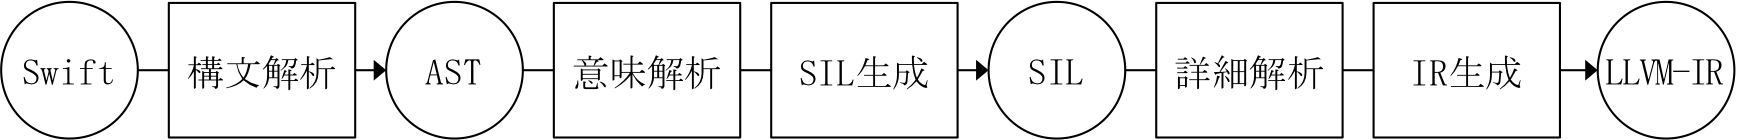
\includegraphics[scale=0.5]{./img/swift_compiler_process.png}
        \caption{Swiftコンパイラの構成}
        \label{img:swift-compiler-process}
    \end{center}
\end{figure}

この図が表現しているのは、Swiftコンパイラのデータ構造を媒介とした各処理ステップの独立性である。
Swiftコンパイラでは各処理ステップで扱うデータ形式を原則としてSwift、AST、SIL、LLVM-IRのいずれかに限定することで処理ステップ間の結合を疎にしている。

以下ではSwiftコンパイラで行われる各処理ステップについて、それぞれの目的とそのために使用されている手法について概説する。
なお、本論文内のSwiftコンパイラについての説明はswift-2.2-SNAPSHOT-2015-12-31-aのリリースにおけるソフトウェアの内容に基づいている。

\subsection{構文解析}
\label{refinement:structure:parser}

構文解析は次の2つの目的のために行われる。

\begin{enumerate}
    \item ただの文字列であるSwiftプログラムを解析して構造を持った抽象構文木(AST)に変換する
    \item プログラムの構文的な誤りを検知して報告する
\end{enumerate}

1つ目の目的を達成するために、SwiftではLL(k)クラスの再帰下降構文解析を手作業で構築して用いている。
この手法についての理解を深めるために、以下では近代的なプログラミング言語に用いられるもう1つの構文解析手法と共にこの構文解析手法について解説する ~\cite{dragonbook}。

\subsubsection{下向き構文解析}

下向き構文解析では、プログラム全体を表現する非終端記号の文法から順により詳細な構成要素に深さ優先で分解していくことによってプログラムを解析する。
Swiftで用いられているLL(k)クラスの再帰下降構文解析は下向き構文解析の1種である。

\vspace{2em}
{\sl\small{TODO: dragonbook P.234のような図を追加}}
\vspace{2em}

再帰下降構文解析は関数によって表現された手続きの集合として構成され、最初の文法を表現する手続きからより詳細な構成要素のための文法を表現する手続きを再帰的に呼び出すことで処理が行われる。
そのため、再帰下降構文解析では文法と実装が明確な対応関係を持っている事が多く、手作業で構文解析器を作成することが比較的簡単である。

\subsubsection{上向き構文解析}

上向き構文解析では、プログラムの字句を先頭から順に読み、具体的な字句をより抽象的な非終端記号へと還元していくことで当てはまる文法を決定していくことでプログラムを解析する。

\vspace{2em}
{\sl\small{TODO: dragonbook P.252のような図を追加}}
\vspace{2em}

上向き構文解析において最もよく用いられているのはLR(1)クラスの構文解析器である。
LR(1)クラスの解析器は多くのプログラミング言語で用いられる文法の殆どを解析できる上、Yaccに代表されるような古くからよく用いられている構文解析器の自動生成ソフトウェアが存在する。
ただし、逆にLR(1)クラスの解析器を手作業で記述するのは容易ではない。
なお、LL(k)クラスの解析器についても構文解析器を自動生成するソフトウェアは存在する~\cite{antlr}が、LR(1)クラスの解析器ほど頻繁に使用されてはいない。

\vspace{2em}

このように構文解析器には複数の設計手法が存在しており、その内の幾つかの手法においては同等の解析能力を保持しているが、どの手法を採用するかによって構文解析器のプログラムは大きく変化する。
また、構文解析器の2つ目の目的であるエラー検知については、その構文解析器が自動生成されるような場合には自動生成されたプログラムの用意するインターフェースによって検知タイミングや検知の難易度が変化する場合がある。
そのため、構文解析器について複雑性を比較する場合には、少なくとも比較を行うコンパイラについても現行のSwiftコンパイラと同じようにLL(k)クラスの再帰下降構文解析を手作業で構築して利用されている必要があると考えられる。

これに加えて、SwiftではSwiftで作成されたライブラリを読み込むためにCやC++におけるヘッダファイルと同じような役割を担う独自形式のモジュールファイルをライブラリ作成時に自動生成しており、構文解析器はこれを解析する役割も担っている。
モジュールファイルの解析は通常のプログラムの解析とは別の関数をエントリ・ポイントとして実行されるために分離して考えることも可能だが、モジュールファイルの解析についても比較を行う場合は、解析にかかる作業量が大きく異なることを避けるために、同様の形式のモジュールファイルを使用している必要があると考えられる。

\subsection{意味解析}
\label{refinement:structure:sema}

意味解析の目的は次のとおりである。

\begin{enumerate}
    \item AST中の変数や関数、型を互いに結びつけ、プログラム全体の整合性を確認する
    \item 開発者によって省略されている情報を補足する
\end{enumerate}

1つ目の目的は主に参照解決と型検査、2つ目の目的は主に型推論を行うことによって達成される。
以下では意味解析の中で行われるこれら3つの処理についてSwiftで使用されている手法と複雑性の比較を行うために統一されるべき設計手法について述べる。

\subsubsection{参照解決}

プログラム中で使用される変数や関数が正確にどこで宣言された変数や関数を指しているかを知ることができるタイミングはその変数や関数がどんな種類であるかに依存する。

例えば、プログラム~\ref{code:explicit-reference}のようなSwiftプログラムでは2行目で参照される変数xが直前の行で宣言されているため、構文解析を行いながら宣言された変数の情報を蓄積しておけば、最短で2行目のxを読んだ直後に変数xの参照を解決できる。
それに対してプログラム~\ref{code:implicit-reference}のように少し複雑化すると、例えばプログラム中5行目の変数s.xの参照を解決するためにはいくつかのステップを踏む必要が出てくる。
このプログラムで変数s.xの参照を解決するためには、まず変数sの参照を解決し、その型が明示されていないためにこれを推論し、クラスSampleのメンバリストから変数xの宣言を探し出すという長大なステップを踏まなければならない。

\begin{lstlisting}[caption=直ちに変数解決が可能である例, label=code:explicit-reference]
let x: Int = 1
print(x)
\end{lstlisting}

\begin{lstlisting}[caption=変数解決までに複数の処理が必要となる例, label=code:implicit-reference]
class Sample {
    let x: Int = 1
}
let s = Sample()
print(s.x)
\end{lstlisting}

このように、参照解決のタイミングはプログラミング言語の仕様によって制限されるが、特に最短のタイミングで解決を行わないといけないということもないため、実装時の簡潔性などを勘案した上で各実装ごとに決定される。
実際、現行のSwiftコンパイラでも参照解決のタイミングはその変数や関数の参照のされ方によってまちまちである。

そのため、比較対象のコンパイラにおいても全く同じタイミングで同じように参照解決が行われるように設計することは容易ではない。
ただし、そのタイミングが異なったとしても比較対象のコンパイラが同等の参照解決能力を持っていることを示すことは不可能ではない。
その場合は、型検査と型推論も含む意味解析部分全体をまとめて比較対象とした上で、意味解析全体を経て最終的に同じように参照解決がなされていることを確認するという形になる。

\subsubsection{型検査・型推論}

SwiftはHaskellやMLなどの関数型言語と同様の非常に強力な型システムを備えており、その型検査と型推論はHindleyとMilnerによる型推論アルゴリズムを拡張したアルゴリズムによって行われている~\cite{swift-type-checker} ~\cite{tapl}。

HindleyとMilnerによる型推論アルゴリズム自体は非常によく知られている上に様々な言語で採用されているが、現行のSwiftコンパイラで行われている独自の拡張は他の型推論を用いる関数型言語と比較してSwiftに特徴的なパラダイムであるオブジェクト指向プログラミングや型パラメータ多相を実現するためのものである。

そのため、型検査と型推論についてコンパイラの比較を行う場合には、HindleyとMilnerによる型推論アルゴリズムを元にしたアルゴリズムを用いた設計にした上で、Swiftが独自に拡張している型についても同等の型推論・型検査能力を備えていることを示す必要がある。
ただし、参照解決の項で述べたように、特定の変数や関数の参照解決を行うために型推論が必要となる場合があるため、型検査や型推論と参照解決を分離して評価することは難しく、どちらかを比較する際には両方を同時に比較せざるを得ないという点には注意する必要がある。

\subsection{SIL生成}

SIL生成は、ASTを分析してより抽象度の低い独自中間言語であるSwift Intermediate Language(SIL)に変換することで最適化などの準備を行うためのステップである。
SILはLLVM-IRをベースとしてループやエラー処理、オブジェクト指向プログラミングのためのクラスの概念などを拡張し、プログラムの意味に基づく詳細なエラー検出などを行い易くした言語である ~\cite{sil}。

SIL生成のステップは特に一般的な手法などに基づいた処理が行われているわけではなく、完全にASTとSILの設計に依存した処理となる。
そのため、SIL生成部分を比較するためには比較するコンパイラにおけるASTの設計を現行のSwiftコンパイラと合わせる必要がある。
ただし実際には、ASTの構造はプログラミング言語の仕様と採用する構文解析手法に依存して決定するため、構文解析手法についても同一のものを選択する必要があるだろう。

\subsection{詳細解析}
\label{refinement:structure:analyze}

詳細解析は、SILを分析してASTのような抽象度の高い状態やLLVM-IRのような抽象度の低い状態では処理しづらい最適化やエラー検出を行うためのステップである。

現行のSwiftコンパイラではSILが包含するコールグラフやクラス階層といった情報を元に最適化やエラー検出を行っており、それらは手法ごとにモジュール化されている。
また、Swiftではメモリ管理の手法として各オブジェクトの作成が要求された際に自動的にメモリを割り当て、不要になったタイミングを検知してメモリを開放するAutomatic Reference Counting方式を用いており~\cite{arc}、そのための処理の挿入などもこの詳細解析で行っている。

詳細解析は複数のアルゴリズムの組み合わせによって構成されているため、比較するコンパイラでもそれぞれの処理について同一のアルゴリズムを採用することで同一の手法を使用した詳細解析を構築することが可能である。

\subsection{IR生成}

IR生成はSILを分析してLLVM-IRを生成することで、低抽象度での最適化や機械語生成を行うための準備を行うためのステップである。

LLVMは統一された中間言語であるLLVM-IRに対する最適化やLLVM-IRから様々なプラットフォーム上で動作可能な機械語へのコンパイルを行うツール群であり~\cite{llvm}、現行のコンパイラはこのLLVMを用いることでコンパイラのバックエンドをフロントエンドから完全に分離している。

LLVMのツールセットは実行可能なソフトウェアや用意されたAPIを通して使用されており、現行のコンパイラではC++で記述されたAPIを用いている。
このAPIには他の言語向けのものも存在するが、LLVMのツールは主にC++で記述されているためにC++のAPIが最も充実しており、現行のSwiftコンパイラはC++のAPIのみで実装されている高度なインターフェースを利用している。
そのため、C++以外の言語で実装されたSwiftコンパイラでは、現行のコンパイラと同じ手法で同じLLVM-IRを生成するように構成することは困難である。

\chapter{Self-host化したSwiftコンパイラ「TreeSwift」の設計と実装}
\label{implementation}

本章では、本研究で実装するSelf-host化したSwiftコンパイラについて、~\ref{refinement:comperable}節における議論を元にその可読性の向上を評価するために必要な設計要件を明らかにし、それを元に行われた実装について説明する。

なお、本研究で実装したSwiftコンパイラは~\ref{refinement:comperable}節で述べた理由から構文解析器のみについて可読性の向上評価が可能となっているが、実際には構文解析器以外の機能も実装されており「TreeSwift」というコードネームが付与されている~\cite{treeswift}。本論文でも現行のApple社によるSwiftコンパイラと簡単に区別するため、本研究で実装したSwiftコンパイラを指してTreeSwiftと記述する。

\section{TreeSwiftの設計}

* 構文解析器のみに絞る
* 構文処理は網羅された仕様書が作成できるので、実際に解析ができるかどうかを網羅的に調べることができるので、できるだけ現行のものと同じになるように実装する
* エラー検知はどれだけ網羅できているかを判断しづらいため、比較の対象から外す
* 同じ手法を徹底することは難しいが、構文解析器全体では同じLL(k)方式を用いる


\section{実装の概要}

* 字句解析には各リテラルの解析を行う決定性有限オートマトンを複数用いている
* モジュール定義にはテキストファイルを使用する
* エラー回復は実装されていない



% \section{構文解析器が満たすべき特徴}
% \label{treeswift:requirements}
%
% Bootstrapを行う上でBootstrap後のコンパイラが満たすべき要件は、基本的にはその言語の仕様を満たしていることと、以前よりも性能が改善されていること以外にはない。
% しかし、本研究では現行のSwiftコンパイラと比較し考察することが目的であるため、評価を行うために必要な同一の特徴を保持している必要がある。
% 以下では、その特徴について述べる。
%
% \subsubsection{LL(k)方式の採用}
%
% 現行のコンパイラの構文解析器と同等の解析力とエラー検出力、拡張性を保持していることを保証するため、TreeSwiftでもLL(k)方式の構文解析器をSwiftで書き下すことによって実装を行う。
%
% \subsubsection{構文解析以外の部分の分離}
%
% 現行のコンパイラとの比較時に比較箇所が行う処理の差が出ないようにするため、型の推論や検査など構文解析以外の部分を構文解析器から分離する。
%
%
% \section{実装の概要}
%
% 本節では~\ref{treeswift:requirements}節で示した特徴を満たしながら、TreeSwiftがどのように実装されているかを説明する。
%
%
% \subsection{構文解析機能}
%
% ソースコードの構文を解析し、ASTにまとめ上げる処理は字句解析と構文解析の2つのステップに分けることができる。
%
% \subsubsection{字句解析}
%
% TreeSwiftでは図%~\ref{img:treeswift-lex} TODO
% のように、入力となるソースコードの文字を1字ずつ読みながら分類し、リテラルや識別子、予約語といった文字数の定まっていないトークンについてはそれぞれに専用の状態遷移機械によって生成する。
%
% \subsubsection{構文解析}
%
% 解析に使用する構文はApple社の提供するSwiftの公式ドキュメント~\cite{swift-grammar}にある構文をベースとするが、本資料は多くの誤りを含んでおりかつLL(k)形式では解析不可能な左再帰を含んでいるため、それらを修正した独自の構文定義を使用している。
%
% また、TreeSwiftでは~\ref{explain-swift:structure:parser}節で述べていたような現行のSwiftコンパイラが判断できていない構文についても、独自の構文定義の追加によって構文的に分類・区別している。
% そのため、TreeSwiftでは全ての構文について構文解析が完了した時点で曖昧性が排除されている。
%
%
% \subsection{参照解決機能}
%
% 変数や型などの参照を解決する機能の実現には、スコープを管理し、解決しなければならない。
% また、参照解決を行うタイミングもその言語仕様に合わせた選択が必要となる。
%
% \subsubsection{参照解決のタイミング}
%
% TreeSwiftでは~\ref{explain-swift:structure:parser}節で述べた現行のSwiftコンパイラの参照解決とは異なり、構文解析中には一切の参照解決を行わない。
% そのため、構文解析が完了して参照解決を行う際にはすでにすべての参照解決が可能であることが保証されており、参照解決を構文解析の本体から分離することが可能となっている。
%
% \subsubsection{スコープ解決}
%
% TreeSwiftにおけるスコープの解決は構文解析時にASTとは別に構築されるスコープツリーを用いて行う。
%
% スコープツリーでは分岐やループ、複合型の宣言などに伴って切り替わるスコープの入れ子構造を木として表現し、木の各ノードがそのスコープ内で宣言された変数や関数、型などをメンバとして保持する。
% また、木の各ノードは後の参照解決のためにスコープ内で参照された変数や関数、型などの情報も保持する。
%
% この構造により、参照解決時には木の各ノードを走査し、各参照情報についてその直近の親ノードから順に参照の対象がメンバとして含まれているかを遡って確認していけば、参照解決を行うことができるようになる。
%
% \subsubsection{曖昧な構文の解決}
%
% また、糖衣構文などを提供するために構文の曖昧性を残しているのもSwiftの特徴である。
% 例えば、プログラム~\ref{code:ambiguous}のような構文はSwiftの構文定義に則った全く正しいコードだが、一般的なアプローチでは正しく解析することができない。
% xの後に続く\{がxの引数のクロージャの始まりなのかif文の本体の始まりなのかは、xが引数としてクロージャを取る関数であることを解析機が知っていなければ決定できず、かつそのxはこれから解析を行う他のファイルなどに宣言されている可能性があるために、全てのファイルの解析を完了するまでxの参照を解決することはできない可能性があるためである。
%
% \begin{lstlisting}[caption=曖昧な構文を持った正しいSwiftコード, label=code:ambiguous]
% let x: (() -> ()) -> Bool = { f in true }
%
% if x { print("closure") } { print("if") }
% \end{lstlisting}
%
% こうした構文を一切の曖昧性なしに解析するためにはコンパイル対象となるプログラムを参照の解決に必要な回数だけ走査しなくてはならなくなるが、それは少なく見積もっても大変非効率であり、現実的ではない。
% 現状のSwiftコンパイラではこうした曖昧な構文は可能性のあるどちらかの構文に決め打ちして実装されており、もう一方を意図して記述しているプログラマに対しては全く見当はずれのエラーメッセージを提示することとなっている。
%
%
% \subsection{構文解析器のその他の機能}
%
% \subsubsection{エラーの処理}
%
% TreeSwiftの実行中に発見されたソースコードのエラーは構文解析ステップを通して同じ1つのインスタンスによって処理される。
% 構文解析器からはエラーを発見した時点でエラー文の参照と解析対象に関する情報をそのインスタンスに渡す。
% そのエラーが致命的なものであった場合や、エラーを管理するインスタンスに設定された既定値よりも多くのエラーが報告されていた場合は、その時点でSwiftのエラーハンドリング機能を用いて解析中の構文の関数を抜け、エラー表示などの処理を行う。
%
%
% \subsubsection{ライブラリの扱い}
%
% TreeSwiftでは独自のバイナリ形式を使用している現行のSwiftコンパイラとは異なり、標準ライブラリを含むライブラリ内に定義されている変数や関数、型などの情報を保持するモジュール情報ファイルをテキストファイルで管理している。
% それらのライブラリはimport文によって要求された時か、標準ライブラリの場合はプログラマがインプットした全てのソースコードの解析前に一度だけ解析され、一般的なソースコードと同様のASTを形成する。
%
% ただし、ライブラリのモジュール情報ファイルでは複数のファイルにまたがったグローバル変数などの定義は存在しないため、構文解析中に即座に参照解決を行う。
%
% \subsection{構文解析以外の実装}

%%% Local Variables:
%%% mode: japanese-latex
%%% TeX-master: "../bthesis"
%%% End:

\chapter{評価}
\label{evaluation}

本章では、~\ref{implementation}章で述べたTreeSwiftを用いて、現行のSwiftコンパイラとその構文解析器の複雑性に関する比較評価を行う。

また同時に、~\ref{side-effect:swift:demerit}節で懸念点として上がっていたSelf-host化に伴う性能の低下という副作用についても、実際にその可能性が存在するかどうかを両コンパイラの構文解析器の性能を比較することで評価・考察する。

\section{構文解析器の複雑性評価}
\label{evaluation:complexity}

本節では2つのSwiftコンパイラの構文解析器について、~\ref{readability:evaluation}節で述べた手法から使用する手法を決定し、実際にその手法を用いて複雑性を計測・比較し、結果について考察する。

\subsection{評価手法}
\label{evaluation:complexity:method}

~\ref{implementation:parser}節で述べたように、TreeSwiftの構文解析器には現行のSwiftコンパイラと異なる部分がある。
そこで、本研究ではできるだけ同じ機能部分についてのみの比較を行うために、両コンパイラの構文解析器のソースコードのうちでも、特定のSwiftプログラムをコンパイルした際に実行された箇所だけを抜き出し、その部分について複雑性の計測と比較を行う。

\vspace{2em}
{\sl\small{TODO: 図で説明する}}
\vspace{2em}

この制限により、比較されるソースコードは共に全く同じ構文を対象としたものだけに限定され、さらに用いるSwiftプログラムを構文的な誤りを含まないものにすることで、エラー回復などの両構文解析器間で手法が異なっている部分を評価対象から外すことができる。
また、同様に扱うファイル形式が異なることが複雑性の差に影響する恐れのあるモジュール解析についても、評価の対象に含まない。
モジュール解析部分はソースコード内で本体プログラムの解析とは独立した関数から行われるため、その分離は容易である。

次に、ソフトウェアの複雑性を評価する手法として~\ref{readability:evaluation}節ではLOC、FP、HCM、CCMという4つの手法について紹介したが、これらの信憑性について大きな差はないため、本節では特に計測しやすいLOCをベースとした評価のみによって複雑性の比較を行う。
LOCには、その各行が表している内容によって行を分割することにより、計測の結果をさらに深く考察できるというメリットも有る。

これらを踏まえ、本研究では具体的に表~\ref{table:complexity-measure}の手順に従って構文解析器の複雑性の計測を行う。
また、この手順によって得られる値とその値に期待される意味は表~\ref{table:complexity-value}のとおりである。

\begin{table}[!hbtp]
    \begin{center}
        \caption{複雑性の計測手順}
        \begin{tabular}{|p{0.05\linewidth}|p{0.9\linewidth}|}
            \hline
            順番 & 手順 \\
            \hline
            \hline
            1 & 計測対象のコンパイラをデバッグ情報付きでコンパイルする \\
            \hline
            2 & コンパイラをデバッガで読み込み、ソースコード中のすべての行にブレークポイントを追加する \\
            \hline
            3 & ブレークポイントは対応する機械語の存在する行でのみ設定されるため、その数を数える \\
            \hline
            4 & コンパイラを構文解析のみ実行するオプション付きで用意したSwiftプログラムに対して実行し、1度でもヒットしたブレークポイントに印をつける \\
            \hline
            5 & 印のついたブレークポイントの数を数える \\
            \hline
        \end{tabular}
        \label{table:complexity-measure}
    \end{center}
\end{table}

\begin{table}[!hbtp]
    \begin{center}
        \caption{計測によって得られる値}
        \begin{tabular}{|p{0.475\linewidth}|p{0.475\linewidth}|}
            \hline
            値 & 値に期待される意味 \\
            \hline
            \hline
            ブレークポイントが設定された行数 & ソースコード中の実行可能な行数 \\
            \hline
            印のついたブレークポイントの数 & 用意したSwiftプログラムのコンパイルに使用された実行可能な行数 \\
            \hline
        \end{tabular}
        \label{table:complexity-value}
    \end{center}
\end{table}

\subsection{計測}
\label{evaluation:complexity:measurement}

計測に使用したプログラムの全文は付録~\ref{appendix:whole-program}に付した。
プログラムではSwiftの用意する構造体、列挙体、クラス、プロトコル、変数、関数、ループ、分岐、エラー処理などの構文を満遍なく利用している。

計測時に使用した各コンパイラの情報を表~\ref{table:compiler-environment}、計測の結果を表~\ref{table:complexity-result}に示す。
なお、ここでは~\ref{table:complexity-value}で示した値に加え、後の考察のために行をその特徴によって分けた場合の値も記述している。

\begin{table}[!hbtp]
    \begin{center}
        \caption{計測に使用したコンパイラの情報}
        \begin{tabular}{|p{0.2\linewidth}|M{0.375\linewidth}|M{0.375\linewidth}|}
            \hline
            情報 & TreeSwift & 現行のSwiftコンパイラ \\
            \hline
            \hline
            バージョン & - & swift-2.2-SNAPSHOT-2015-12-31-a \\
            \hline
            実行ファイルの生成に用いたコンパイラ & Apple Swift version 2.1.1 & clang version 3.8.0 \\
            \hline
            行数のカウントに使用したデバッガ & \multicolumn{2}{|c|}{lldb-340.4.119} \\
            \hline
        \end{tabular}
        \label{table:compiler-environment}
    \end{center}
\end{table}

\begin{table}[!hbtp]
    \begin{center}
        \caption{計測の結果}
        \begin{tabular}{|p{0.2\linewidth}|M{0.375\linewidth}|M{0.375\linewidth}|}
            \hline
            計測項目 & TreeSwift & 現行のSwiftコンパイラ \\
            \hline
            \hline
            ソースコード中の実行可能な行数 & & \\
            \hline
            Swiftプログラムのコンパイルに使用された実行可能な行数 & & \\
            \hline
        \end{tabular}
        \label{table:complexity-result}
    \end{center}
\end{table}

\subsection{考察}


\section{構文解析器の性能評価}

本節では2つのSwiftコンパイラの構文解析器について、その性能を計測する手法について整理した上で実際にその手法を用いて性能を計測・比較し、結果について考察する。

\subsection{評価手法}

* 速度とメモリ使用量を計測する

\subsection{計測}

\subsection{考察}

%%% Local Variables:
%%% mode: japanese-latex
%%% TeX-master: "../thesis"
%%% End:

\chapter{結論}
\label{conclusion}

本章では、本論文の結論と今後の展望を示す。

\section{本研究の結論}

本研究では、Swiftコンパイラのソースコード可読性をSelf-host化によって向上させることを目的として、Self-host化したSwiftコンパイラを実装し、現行のコンパイラとその可読性を比較した。
両コンパイラの構文解析器について、Swiftのチュートリアル中で用いられている7つのサンプルプログラムを解析するために必要な箇所を抜き出してその行数を比較した結果、特にSwiftの持つパターンマッチなどの機能によってSelf-host化したコンパイラの方が6つのプログラムにおいてより高い可読性を持っていることが示された。
このことから、Self-host化によってSwiftコンパイラのソースコード可読性の向上が充分に期待できるが、その可読性の向上はSwiftの構文が主要因となっているため、他の既に高級言語でコンパイラが記述されている言語においては同様の手法を用いたとしても同じような結果を得られるとは限らない。

\section{今後の展望}

\subsection{構文解析器以外の比較}

構文解析以降の処理ステップについては、その処理が1つ前のステップの影響を受けるため、~\ref{evaluation:measure}節でASTファイル群について可読性が向上しているかどうかを判断できなかったように、本研究の手法ではうまく可読性の比較を行えない可能性が高い。

しかし、コンパイラの他の処理ステップには~\ref{refinement:structure}節で述べたように構文解析器とは異なる様々なアルゴリズムやデータ構造が使用されており、その中には構文解析器のようにSwiftの構文による可読性の向上が充分に発揮されない箇所が存在する可能性もある。

そのため、実際にSwiftコンパイラの全体をSelf-host化するか否かを判断するためには、他の処理ステップについても何らかの手法を用いて評価を行っていく必要があるだろう。

\subsection{継続的な比較}

Swiftは現在も破壊的な変更を含む活発な仕様変更の相次ぐ言語であり、今後のバージョンの仕様で比較した場合は、可読性についての評価結果も変化する可能性がある。
そのため、確かにSwiftに対してSelf-host化が十分な可読性の向上をもたらすことを判断するためには、今後のバージョンでも継続的に同様の比較を行い、その変化を見る必要がある。

%%% Local Variables:
%%% mode: japanese-latex
%%% TeX-master: "../thesis"
%%% End:

\chapter*{謝辞}
\addcontentsline{toc}{chapter}{謝辞}
\label{thanks}

本論文の作成にあたり、ご指導いただきました慶應義塾大学環境情報学部教授村井純博士、同学部教授中村修博士、同学部准教授 Rodney D. Van Meter III 博士に感謝致します。

研究について日頃からご指導頂きました松谷健史氏、空閑洋平氏に感謝致します。
研究室に所属したばかりの頃から本研究に至るまで、特定の分野にこだわらない広い視点から絶えず多くのご指導をいただきました。
本研究を卒業論文としてまとめることができたのも両氏のおかげです。重ねて感謝申し上げます。

研究室を通じた生活の中で多くの示唆を与えてくださった髙橋俊成氏、Arch研究グループの皆様に感謝します。

また、徳田・村井・楠本・中村・高汐・バンミーター・植原・三次・中澤・武田合同研究プロジェクトの皆様に感謝致します。

%%% Local Variables:
%%% mode: japanese-latex
%%% TeX-master: "../yummy_bthesis"
%%% End:

\appendix
\chapter{TreeSwiftの実装における留意点}

本研究で現行のSwiftコンパイラとの比較に用いたTreeSwiftは実際には本論文の動機として紹介されているSwiftのオープンソース化よりもずっと以前から実装が進められていた。
つまりTreeSwiftはApple社の実装の詳細を知ること無くSwiftコンパイラを実装していたにも関わらず、結果的に構文解析器において同じ手法を採用していたということである。

本付録では、本論文の論旨とは一切関係ないものの、そうしたTreeSwiftの設計や実装を行う上で見つけた幾つかの気付きとそこから得た知見について、TreeSwiftの実装を解説しながら紹介する。
本付録における情報は、本論文で提案しているようにSwiftコンパイラをSelf-host化する際はもちろん、Swiftを含む近代的な言語のコンパイラを設計する際などにも役立つだろう。


\section{SwiftでSwiftコンパイラを記述する上での障壁}

Apple社のSwiftコンパイラとTreeSwiftとの一番大きな差は実装開始当初から変わらず、Self-host化されているという点にある。
しかし、SwiftはもともとApple社の提供するフレームワークを用いた特定のプラットフォーム向けのアプリケーションを記述するためのドメイン特化言語のように発表されていた。
そのため、そもそもSwiftにはコンパイラを実装するために十分な機能が用意されていない可能性があり、まずはSwiftコンパイラの各ステップで行われている処理を明らかにして、それらの処理がSwift言語でも実現できるかどうかを考察する必要があった。

実際にそうした考察を行うと、Swiftコンパイラで行われている処理の中にはSwiftだけでは実現が困難な特に大きな2つの処理が存在していた。
本節ではそれらについて、その処理の実装が難しかった原因とTreeSwiftで取った解決方法を紹介する。

\subsection{ファイル入出力}

まず、最初に問題となるのはファイルの入出力である。
コンパイラでは言わずもがな、プログラムのソースファイルを入力し、中間言語ファイルや場合によっては特定の形式のバイナリファイルなどを出力する必要がある。
また、ほとんどのコンパイラではソースファイルにエラーや警告が見つかった場合にその原因箇所をユーザに知らせることを目的として、字句や構文を表現する各オブジェクトにそのオブジェクトが対応するソースコード中の場所を保持させる。
その情報から実際のコードをスムーズに参照しエラーなどと一緒に表示するには、ファイル内の特定箇所に直接アクセスするインターフェースが必要となる。
しかし、これらの機能はSwiftの標準ライブラリでは提供されていないか不十分であった。

そのため、TreeSwiftではApple社がSwiftコンパイラと一緒に提供しているDarwinをベースとした環境のC言語の標準ライブラリをSwiftのライブラリであるかのように利用できるDarwinモジュールを用い、freadやfseekなどの関数をラッピングしたクラスを作ってファイルの入出力処理を行っている。

\subsection{LLVMの使用}

次に大きな問題となるのは、Swiftのバックエンドを担うLLVMの使用である。
もちろん、LLVMはコンパイラのバックエンドを実現するための1つの方法でしか無いので、TreeSwiftでもこれを採用しなければならないということはない。
しかし、Swiftの文法について詳細に見ると、その中にはLLVMを使用することが前提であるかのように感じるものがいくつかあることに気づく。
その典型的な例が、Swiftのアクセスレベル修飾子とLLVM-IRのリンケージタイプとの類似性である。

表~\ref{table:linkage-access-level}にSwiftの3つのアクセスレベル修飾子とLLVMの3つのリンケージタイプ~\cite{llvm-man}およびそれらの意味を似ている物同士で並べて示した。
SwiftにおけるファイルをLLVMにおけるモジュール、SwiftにおけるモジュールをLLVMにおけるオブジェクトファイルと読み替えれば、それぞれのアクセスレベル修飾子とリンケージタイプが明らかな対応関係にあることが分かる。
つまり、Swiftのアクセスレベル修飾子はLLVMをバックエンドに用いた際にその実装が簡単になるように設計されていると見れる。

\begin{table}[!hbtp]
    \begin{center}
        \caption{Swiftのアクセスレベル修飾子とLLVMのリンケージタイプの類似性}
        \begin{tabular}{|p{0.2\linewidth}|p{0.275\linewidth}||p{0.2\linewidth}|p{0.275\linewidth}|}
            \hline
            \multicolumn{2}{|c||}{Swiftのアクセスレベル修飾子} & \multicolumn{2}{|c|}{LLVMのリンケージタイプ}\\
            \hline
            名前 & 意味 & 名前 & 意味\\
            \hline
            \hline
            private & 修飾された要素は同一ファイル内からのみアクセス可能 & private & 修飾されたグローバル値は同一モジュール内からのみアクセス可能\\
            \hline
            internal & 修飾された要素は同一モジュール内からのみアクセス可能 & internal & 修飾されたグローバル値は同一オブジェクトファイル内からのみアクセス可能\\
            \hline
            public & 修飾された要素は外部モジュールからでもアクセス可能 & available\_externally& 修飾されたグローバル値はどこからでも参照可能\\
            \hline
        \end{tabular}
        \label{table:linkage-access-level}
    \end{center}
\end{table}

こうした類似点が他にも多数存在しているため、TreeSwiftにおいてもそのバックエンドにLLVM以外のプラットフォームを用いたり、バックエンドまで自作するような考え方はなかった。
ただそうすると、LLVMのメインとなるAPIがC++で提供されており、CやPython向けに提供されているAPIがその機能面においてC++のものよりも劣っているという点が問題になる。

TreeSwiftでは最初、この問題に対してLLVMのC++用APIをラップしたObjective-Cのライブラリを作成し、そのライブラリをSwiftから読み込むことで対処しようとした。
Objective-CにはC++と、SwiftにはObjective-Cとの相互運用性があるため、これらを組み合わせることで問題を克服できると考えていたからである。
しかし、実際にはObjective-Cのカプセル化機構ではバックグラウンドでC++のライブラリ内に定義されたC++のオブジェクトを用いながらも、それらを一切含まない純粋なObjective-Cだけのインターフェースを備えたラッパークラス群を定義することが難しく、そのコストの高さからこのアプローチは不採用に終わった。

結果として、現在のTreeSwiftではLLVMのC言語用APIを直接用いてSwiftからLLVMを使用している。
LLVMのC言語用APIにおいてSwiftコンパイラを設計する上で充分な機能が提供されているか、という点には未だ不安が残っているが、TreeSwiftの実装と同時期に作られたRuby言語に似たコンパイラ型言語であるCrystal~\cite{crystal}がBootstrapするためにこのAPIを使用しているという例もあるため、根本的な欠陥はないであろうと考え、実装に使用している。


\section{Swiftの文法と実装に対する示唆}

Swiftの文法はオープンソース化以前より公式ドキュメント~\cite{swift-grammar}上でBNFに近い形式の構文で公開されており、それを参照することでSwiftのユーザは文法の詳細までを知れるようになっている。
しかし、そこで公開されている文法は単にSwiftの文法を解説するためのドキュメントでしかなく、実装されている文法とは細部で異なる部分が多々存在している。
そのため、TreeSwiftを実装するにあたってはまずドキュメントの文法を全て書き写し、文法中の間違いや不適切な点を修正する作業を行う必要があった。

ただ、この修正作業のためにSwiftの文法を細かく確認したことで得られたSwiftの文法に関する知見は多く、結果としてそれらの知見が構文解析器を実装する上で重要な幾つかの判断を助けることとなった。
本節ではそうした知見の中から特にTreeSwiftの設計に影響を与えた2つの例を紹介する。

\subsection{文法の曖昧性と構文解析器の文法クラス}

Swiftの基本的な文法はCやC++、Objective-Cなどの俗にC-Familyと呼ばれるプログラミング言語に類似しているが、それらの言語とは異なり、Swiftの文法はプログラマにコンパイラが構文解析を行うための記述を強いないように注意深く設計されている。
Swiftでは文の終わりを示す";"や制御構文の条件式の前後に"("と")"を付けることを強制しないし、順に実行される手続きの集まりは制御構文内・関数定義内・無名関数内などのどこに書かれるかにかかわらず、"\{"と"\}"で囲うことで表される。
しかし、こうしたプログラマ中心の設計は当然のことながら、他のC-Family言語のコンパイラでは問題になっていなかった箇所で構文の曖昧性を生み、コンパイラの仕事を増やしている。

例えば、プログラム~\ref{code:ambiguous}はSwiftの文法に則った全く正しいプログラムだが、このプログラムを曖昧性無く解析するのは非常に難しい。
2行目のifから始まる文を解析するためには、xの後に続く"\{"がxの引数のクロージャの始まりなのかif文の本体の始まりなのかを判断するために、xの参照を解決した上でその型を知る必要がある。
このプログラムにおいては直前にxの宣言があるためにxの参照を解決することはできるが、xの型は明示的に注釈されていないため、これを推論する必要が出てくる。

\begin{lstlisting}[caption=曖昧な構文を持った正しいSwiftプログラム, label=code:ambiguous]
let x = { (f: () -> Bool) in f() || true }
if x { print("closure argument") } {
    print("if body")
}
\end{lstlisting}

ではここで、制御構文の条件式の後に"\{"と"\}"で囲まれた手続きの集まりが2度以上現れるような曖昧性のある構文に当たった場合だけ、条件式の型推論を先に行うように構文解析器を設計したとする。
その設計を前提に考えると、今度はプログラム~\ref{code:complex-incorrect}のような複数のファイルにプログラムが分かれている多少複雑な例を解析する際に問題が生じる。
\begin{lstlisting}[caption=特定のアプローチではエラーの検出に多大な計算量を要する誤ったSwiftプログラム, label=code:complex-incorrect]
// class.swift
class Sample {
    let a = true
}

// function.swift
func f() {
    let s = Sample()
    if s.a {
        print("if body")
    } {
        print("missing else keyword body")
    }
}

// main.swift
f()
\end{lstlisting}

この例では2$\sim$4行目、7$\sim$14行目および17行目がそれぞれclass.swift、function.swift、main.swiftという3つのファイルに分かれているものとしているが、その11行目、function.swift内の5行目にif文に続くelse文に必要なキーワード"else"を書き忘れているというバグがある。
そのため、実際にプログラムの解析を始めると、このバグにより現在想定している構文解析器は9$\sim$13行目の文を曖昧性のある制御構文とみなし、s.aの型を推論しようと試みる。
しかし、この変数sのクラスSampleはclass.swiftという別ファイルで宣言されているため、そのクラスのインスタンス変数であるaの型を解決するためには、function.swiftよりもclass.swiftを先に解析しておく必要があり、ここで問題が生じる。
Swiftにおいてmain.swiftと命名されたファイル以外のファイルについて名前の規定はなく、それらの解析順を誘導することはできないからである。
つまり、現在想定している構文解析器においてこのプログラムから正しくエラーを検出するためには、曖昧性の原因となっている式とその式に関連するすべての項を正しく型付けできるか型付けできないことが明らかになるまで、main.swift以外の全ファイルを繰り返し解析し直す必要があるのだ。
この解決方法が解決したい問題に対して非常に複雑であり、かつ構文解析器の処理時間を必要以上に引き伸ばしてしまうことは明らかである。

そのため、こうしたSwiftの曖昧な構文では正確に解析することを諦め、曖昧性のある構文としてエラーにするか、どちらかの構文として決め打った解析のみを行うように構文解析器を設計する必要がある。
ただ、こうした設計を実現するためには、構文解析器で採用できる実装手法が限られてくる。

まず、先述のような曖昧性のある文法BNFなどで記述し、その構文解析器を完全に自動生成することは現実的ではない。
現在主に用いられている構文解析器の自動生成ソフトウェア~\cite{antlr}は解析対象の言語に曖昧な文法が含まれず、最悪の場合でもプログラム中の全ての字句を先読みすれば適用する文法が決定できるという前提のもとに設計されているからである。

さらに、たとえ一部であっても構文解析を手作業で書き下すとなると、~\ref{refinement:structure:parser}節でも述べたように、上向き構文解析を用いることは難しい。

そのため、近年のコンパイラで用いられているようなアルゴリズムを用いるのであれば、Swiftの構文解析器は下向きかつ任意個の字句を先読みするLL(k)などに代表される文法クラスのものとなり、かつそれを完全に手作業で書き下すか、一部のみについて自動生成を用いる形となる。

そうしたSwiftの文法の持つ性質から考えてTreeSwiftではLL(k)クラスの再帰下降構文解析を手作業によって書き下すこととなったので、Apple社のSwiftコンパイラにおいても全く同じアプローチの構文解析器が実装されていたという事実は驚くに値しないかもしれない。
しかし、Apple社の提供するドキュメントではSwiftの文法が下向き構文解析で解析不可能な左再帰を含んで記述されているところを見ると、文法の持つ性質を注視せずに構文解析器を設計し始めていた場合にはここで示したような問題と真正面からぶつかり、以上に非効率な構文解析器を実装してしまっていた危険性も十分にあったと考えられるのである。

\subsection{変数の宣言とスコープ}


\section{参照解決・型推論・メンバ呼び出しの相互依存性}

現時点のTreeSwiftにおいてまだうまく実装ができていないSwiftの機能として、意味解析のステップにおける相互に依存する参照・型・メンバ呼び出しの解決がある。

~\ref{refinement:structure:sema}節でも言及したように、Swiftではオブジェクト指向プログラミングを採用し、型の省略と関数のオーバーロードを同時に許しているため、特定の関数の参照を解決するためには適切な順で型推論やメンバ呼び出しの解決、関連する他の参照の解決を先に行う必要がある。
さらに、その内の型推論だけに限って見てもSwiftはプロトコルと呼ばれる存在型やジェネリクスと呼ばれる全称型を利用できるようにしており、型同士の関係性を解決を行うプロセスまでもが非常に複雑化している。

これは、他の言語と比較してもかなり欲張った設計である。
よく使われている言語の例で言えば、C++やJava、Scalaは関数のオーバーロードを許すオブジェクト指向言語であるがSwiftのように強力な型推論を提供していないし、OCamlやRustといった関数型言語の色が強いオブジェクト指向言語では強力な型推論を提供している代わりに、完全な関数のオーバーロードを許してはいない。
さらに比較して近年に開発された言語であっても、2005年に登場したHaxe~\cite{haxe-overload}や2011年に登場したばかりのCeylon~\cite{ceylon-overload}はOcamlなどと同様に強力な型推論と引き換えに関数のオーバーロードをその仕様に含めていない。

そこで本節では、この意味解析の設計をSwiftコンパイラを実装する上で特に難易度の高い箇所であると捉え、TreeSwiftを実装する上で遭遇したこの意味解析における難題に繋がる2つの設計上の分岐点について紹介する。

\subsection{参照解決のタイミング}

\subsection{メンバ呼び出しの型解決を行うタイミング}


\renewcommand{\thechapter}{\Alph{chapter}}
\setcounter{chapter}{0}
\vspace{-5mm}


\bibliographystyle{unsrt}\pagestyle{plain}
\bibliography{./bib/cites,./bib/bootstrapping_evidence,./bib/appendix}\pagestyle{plain}
\thispagestyle{empty}%bibtex


\end{document}

%%% Local Variables:
%%% mode: japanese-latex
%%% TeX-master: t
%%% End:
